\documentclass{article}
\usepackage{graphicx}
\usepackage{subcaption}
\usepackage{arxiv} % https://github.com/kourgeorge/arxiv-style
\usepackage{graphicx} % Required for inserting images
\usepackage{amsmath}
\usepackage{biblatex}
\usepackage[hidelinks]{hyperref}
\usepackage{ccicons}

\bibliography{references.bib}

% \newcommand{\ccbync}{
%   \noindent\href{https://creativecommons.org/licenses/by-nc/4.0/}{%
%     
\includegraphics[height=2em]{by-nc.png}%
%     \hspace{0.5em}CC BY-NC 4.0 License}%
% }

\title{Informe Final IPD439 \\
Caracterización de periféricos de señal mixta en microcontroladores}
\author{Sebastián Sánchez (sebastian.sanchezp@usm.cl) }
%\thanks{Este trabajo está licenciado bajo una licencia \href{https://creativecommons.org/licenses/by-nc/4.0/}{Creative Commons Attribution-NonCommercial 4.0 International}  
\includegraphics[height=1.5em]{by-nc.png}.}}
\date{Abril 2026}
\graphicspath{{figures}}
\begin{document}

\maketitle

\section{Resumen}
Este trabajo presenta la caracterización de periféricos de señal mixta de los microcontroladores STM32L476RG utilizando múltiples generadores de señales, tanto digitales cómo análogos. En particular se obtuvieron métricas de corriente continua y alterna para convertidores análogo-digital (ADC) y solo de corriente continua para de convertidores de datos digital-análogo (DAC), la obtención de estas fue mediante el seguimiento de los estándares IEEE correspondientes a la caracterización de ADCs (N°1241) y DACs (N°1658). Los resultados obtenidos muestran fidelidad para el DAC de la STM32 al compararlos con su datasheet, mientras que se aprecian un múltiples errores para métricas del ADC de la STM32 dependiendo del generador de señal utilizado, en ciertas métricas que debiesen ser minimizadas se reportó un valore entre 5 a 10 veces del valor máximo reportado en el datasheet y en ciertas métricas que debiesen ser maximizadas se reportan valores cercanos al 70\% de lo mínimo reportado en el datasheet. Se concluye que se deberá mejorar la rigurosidad en la generación de forma de onda inyectada así como la modificación del filtro de entrada.
\section{Introducción}
En nodos IoT es altamente probable que se requiera el uso de un microcontrolador que posea comunicación inalámbrica (Wi-Fi o Bluethooth), posea periféricos análogos robustos y confiables y tenga un bajo costo unitario. Ante estas restricciones, la toma de decisión de que microcontrolador utilizar se vuelve una tarea ardua la cual dependerá únicamente de horas de lectura de datasheets para poder tomar una decisión informada.\\
La primera opción que uno pensaría ante las restricciones de bajo costo y comunicación inalámbrica serían los microcontroladores de la familia ESP32. Sin embargo, estos son infames por sus convertidores análogos, ya sea por la mala precisión o poca documentación que poseen. Es por esto, que en este trabajo se presenta un avance en
la validación de métricas de los conversores de datos análogo digital (ADC) y comparativa
comparativa entre los convertidores análogos de la tarjeta de desarrollo ESP32 S3 Mini, de aquí en adelante referida solamente como ESP32, y la tarjeta de desarrollo STM32 L476RG, de aquí en adelante referida solamente como STM32, la cual  posee amplia documentación respecto a sus convertidores de datos.\\
Para esto, en las siguientes secciones se presentan las métricas de desempeño extraídas y analizadas para los conversores en cuestión.\\
El resto de este documento se organiza de la siguiente manera: la Sección 3 detalla el marco teórico fundamental, abarcando las arquitecturas de los periféricos, métricas de desempeño, requerimientos de la señal de entrada y consideraciones térmicas. La Sección 4 menciona las normativas adoptadas. La Sección 5 establece los objetivos del proyecto. Posteriormente, la Sección 6 describe la metodología, justificando los instrumentos utilizados y detallando el flujo de medición. Finalmente, la Sección 7 presenta los resultados preliminares obtenidos, dando paso a la Sección 8, donde se exponen las conclusiones derivadas de los resultados.
\section{Marco teórico}
La validación de periféricos de señal mixta exige un alto rigor técnico y analítico, es por esto que antes de empezar a realizar mediciones fue indispensable estudiar los detalles técnicos que sustentan las métricas de desempeño. En las siguientes subsecciones se darán a conocer las arquitecturas que poseen estos periféricos, los fundamentos de las métricas escogidas y obtenidas, las características necesarias de las señales de entrada, las consideraciones térmicas y, finalmente, los protocolos de comunicación utilizados para la obtención de métricas.   
\subsection{Arquitectura del los ADCs}
Los ADCs implementados en la STM32 y ESP32 son de aproximación sucesiva (SAR), esta arquitectura genera N comparaciones de manera sucesiva para una sola medición y, al igual que otras requiere, de un DAC interno para generar estas comparaciones.
\begin{figure}[h]
    \centering
    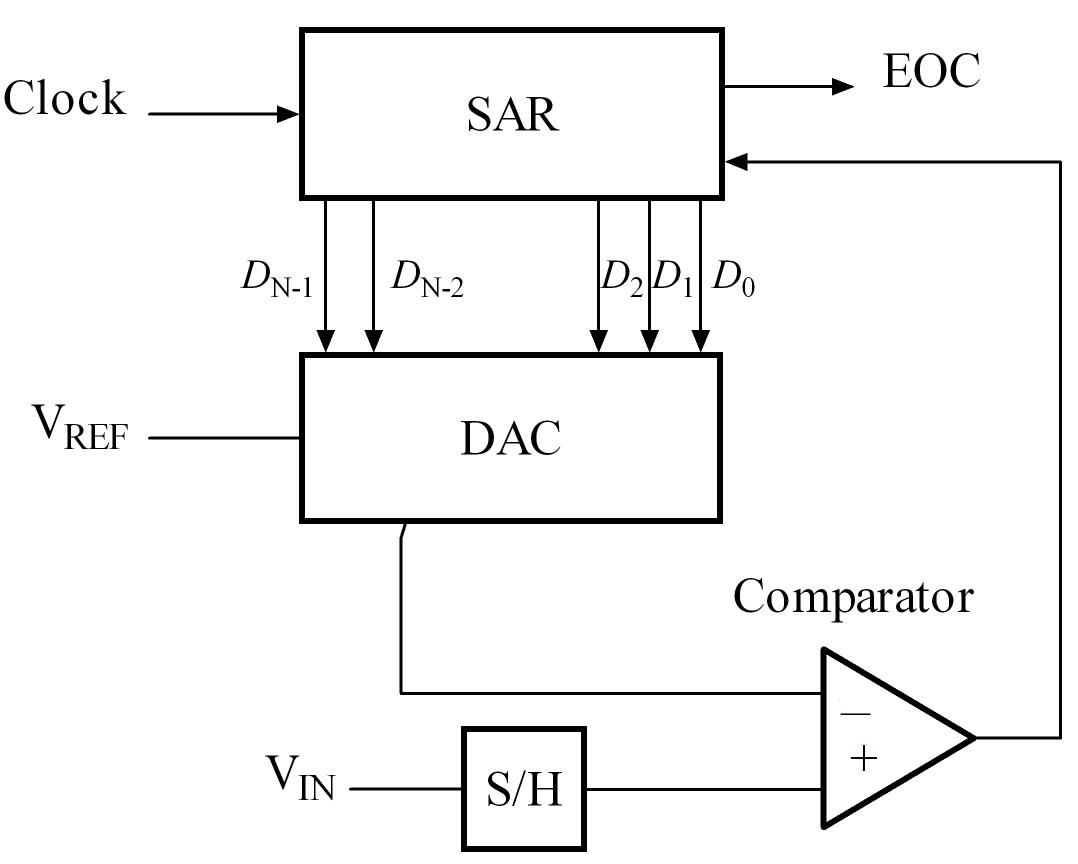
\includegraphics[width=0.3\linewidth]{figures/SA_ADC_block_diagram.png}
    \caption{Arquitectura general de un SAR ADC(imagen obtenida de \href{https://en.wikipedia.org/wiki/Successive-approximation_ADC}{wikipedia}})
    \label{fig:sar}
\end{figure}
\subsection{Arquitectura del DAC}
Antes de ahondar en detalles, es importante destacar que la ESP32 utilizada no posee un Convertidor de datos digital a análogo, por lo que si bien no se podrá realizar una comparación se validaran las métricas de desempeño de este periférico de todas formas.
\\
La arquitectura de los DAC implementados en la STM32 posee el nombre R2R, esta arquitectura recibe este nombre debido a que solamente se utilizan resistencias de valor R y 2R. Es importante notar que estas resistencias vienen integradas dentro del chip, por lo que están sujetas a errores de matching, esto quiere decir que una resistencia diseñada de valor R tendrá una impedancia distinta a otra resistencia de las mismas características, y debido a su baja cantidad de resistencias, esta arquitectura es propensa a generar una salida no lineal.
\begin{figure}[h]
    \centering
    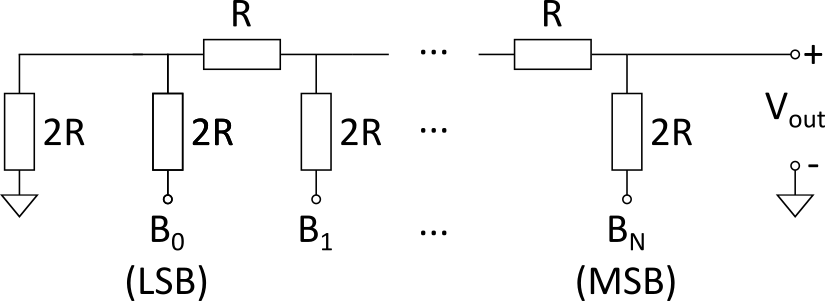
\includegraphics[width=0.5\linewidth]{figures/R2R_DAC.png}
    \caption{Arquitectura del DAC utilizado por la STM32}
    \label{fig:r2r}
\end{figure}
En la Figura \ref{fig:r2r} se puede visualizar la arquitectura descrita. Finalmetne, el voltaje $V_{out}$ puede ser descrito mediante la ecuación \ref{eq:r2r}, con $V_{ref}$ siendo el Voltaje de alimentación (3.3 V) y N el número de bits correspondientes a la resolución.
\begin{equation}
    V_{out}=\frac{V_{ref}}{2^N}\cdot(\sum^{N-1}_{i=0} B_i\cdot 2^i)
    \label{eq:r2r}
\end{equation}
\subsection{Métricas de desempeño}
La caracterización completa y apropiada de estos periféricos representa un trabajo cuyo alcance excede el margen temporal de este proyecto; por lo tanto, se seleccionaron siete métricas de desempeño clave. De estas, cuatro corresponden a parámetros de corriente continua y tres a pruebas de corriente alterna. Estas métricas permiten evaluar la linealidad de los periféricos, el rango de error esperado, la precisión porcentual y su robustez ante el ruido.
\begin{itemize}
    \item \textbf{Error de offset:} Corresponde a la desviación de la transferencia real respecto a la ideal en el primer código de transición. Se mide cuando la entrada debería representar el valor del bit menos significativo (LSB).
    \item \textbf{Error de ganancia:} Representa la diferencia de pendiente entre la característica de transferencia real y la ideal, una vez compensado el error de offset.
    \item \textbf{DNL (No Linealidad Diferencial):} Es la desviación del ancho de un paso de código real respecto al paso ideal de 1 LSB. Matemáticamente, para un código $k$, se expresa como:
    \begin{equation}
        DNL(k) = \frac{V_{step}(k) - V_{LSB}}{V_{LSB}}.
    \end{equation}
    Un valor de $-1$ LSB indicaría la presencia de códigos perdidos (\textit{missing codes}).
    \item \textbf{INL (No Linealidad Integral):} Representa la desviación máxima de la curva de transferencia real respecto a una línea recta ideal (generalmente calculada mediante el método de puntos extremos o mejor ajuste). Se puede entender como la acumulación de los errores diferenciales:
    \begin{equation}
        INL(k) = \sum_{i=1}^{k} DNL(i).
    \end{equation}
    \item \textbf{THD (Total Harmonic Distortion):} Es la razón entre la raíz cuadrada de la suma de los cuadrados de las componentes armónicas y la amplitud de la frecuencia fundamental.
    \begin{equation}
        THD=\frac{\sqrt{\frac{1}{M^2}\sum_{h} |X[f_h]|^2}}{A_{rms}}.
    \end{equation}
    \item \textbf{SNDR o SINAD (Signal-to-Noise and Distortion Ratio):} Es la relación, expresada en decibeles, entre la potencia de la señal fundamental y la suma de la potencia del ruido más todas las componentes armónicas de distorsión.
    \begin{align}
        SINAD_{dB}&= 20 \log_{10}\left( \frac{A_{rms}}{NAD} \right),\\
    NAD&=\frac{1}{\sqrt{M(M-3)}}\cdot\sqrt{\sum_mX_{avm}^2[f_m]}\nonumber .
    \end{align}
    \item \textbf{ENOB (Effective Number of Bits):} Representa la resolución real del sistema considerando el ruido y la distorsión, permitiendo comparar el desempeño del periférico real frente a un conversor ideal.
    \begin{equation}
        ENOB=\frac{SINAD_{dB}-1.76}{6.02}
    \end{equation}
\end{itemize} \vspace{-2mm}
\subsubsection{Significado de variables}
A continuación, se detalla el significado de las variables utilizadas en las expresiones matemáticas anteriores, basadas en el estándar IEEE 1241:
\begin{itemize}
    \item $k$: Índice numérico del código digital evaluado.
    \item $V_{step}(k)$: Ancho del escalón de voltaje analógico medido para la transición del código $k$.
    \item $V_{LSB}$: Ancho del escalón de voltaje ideal correspondiente a un bit menos significativo ($V_{FS}/2^N$).
    \item $M$: Número total de muestras en el registro de datos capturado.
    \item $X[f_h]$: Magnitud de la Transformada Discreta de Fourier (DFT) evaluada en el bin correspondiente a la frecuencia de la $h$-ésima armónica.
    \item $A_{rms}$: Valor cuadrático medio (RMS) de la amplitud de la señal analógica fundamental inyectada.
    \item $NAD$: Voltaje RMS equivalente al ruido y la distorsión residual (Noise and Distortion).
    \item $X_{avm}[f_m]$: Magnitud promediada del espectro en los bines de frecuencia que no corresponden a la señal fundamental ni a la componente DC.
\end{itemize}
\subsection{Señal de entrada}
Para poder caracterizar de manera correcta los periféricos, se debe tener en cuenta que uno de los factores más importantes es la selección de la señal inyectada, pues corroborar métricas con una señal cuyo ruido inherente corresponde al 10\% de la amplitud máxima, equivaldría cómo mínimo una pérdida de 3.3 bits al no considerar distorsión.
\subsubsection{Selección de frecuencia de entrada}
La selección de la frecuencia de la señal de entrada no tiene mucha ciencia en las mediciones de corriente continua, por lo que en este caso se consideró como corriente continua cualquier señal de entrada cuya frecuencia esté entre 1 a 10 Hz.\\
Contrariamente a las mediciones de corriente continua, en corriente alterna la correcta selección de la frecuencia de entrada es un paso crítico. Esta debe ser coherente con la frecuencia de muestreo del convertidor de datos ($f_s$) para garantizar que se capture un número entero y exacto de ciclos de la señal, evitando así el fenómeno de fuga espectral (spectral leakage) al aplicar la Transformada Rápida de Fourier (FFT). Para cumplir con la condición de muestreo coherente, la frecuencia de la señal de prueba ($f_{in}$) se rige por la siguiente relación:
\begin{equation}
    f_{in} = \frac{J}{M} f_s.
\end{equation}
Donde $M$ es el número total de muestras capturadas en el registro y $J$ es el número entero de ciclos de la onda senoidal contenidos en dicha captura. Para asegurar que el ADC evalúe diferentes códigos a lo largo de la prueba y no repita el muestreo en la misma fase geométrica de la onda, el valor de $J$ debe ser un número primo impar. Al asegurar que $J$ y $M$ son mutuamente primos, cada una de las muestras tomadas corresponderá a un punto único de la señal análoga.
\\
\subsubsection{Selección de filtro antialiasing}
La caracterización de parámetros dinámicos, como el SINAD y el ENOB, asume que la señal de estímulo inyectada al ADC es una onda senoidal espectralmente pura. Sin embargo, los generadores de señales comerciales introducen ruido térmico de banda ancha y distorsión armónica intrínseca que, de no ser mitigados, se reflejarán negativamente en las métricas del microcontrolador, limitando la medición al rendimiento del instrumento y no al del silicio bajo prueba.
\\
Para evitar el solapamiento espectral (aliasing) de estas componentes de alta frecuencia en la banda base digital, se implementó un filtro pasa-bajos RC pasivo de primer orden en la entrada del ADC. El diseño consta de una resistencia en serie de $50\ \Omega$, acoplada a la impedancia de salida del generador, y un capacitor de derivación de $1\ \mu\text{F}$. Esta configuración establece una frecuencia de corte ($f_c$) calculada mediante la expresión:\\
\begin{equation}
    f_c = \frac{1}{2\pi R C}.
\end{equation}
Evaluando los componentes, se obtiene una frecuencia de corte aproximada de $3.18\text{ kHz}$.
\subsection{Variaciones de Temperatura}
Es importante notar que la temperatura juega un rol crucial a la hora de generar las pruebas, pues debido a la naturaleza de los semiconductores, sus parámetros intrínsecos son altamente dependientes de las fluctuaciones térmicas. En la caracterización de periféricos de señal mixta como ADCs y DACs, el incremento de la temperatura de la pastilla de silicio impacta directamente en el desempeño estático y dinámico a través de diversos mecanismos físicos:
\begin{itemize}
    \item \textbf{Deriva de la Referencia de Voltaje (\textit{Voltage Reference Drift}):} La tensión de referencia ($V_{REF}$) interna, generalmente implementada mediante un circuito de \textit{bandgap}, sufre una variación en su coeficiente de temperaturamedido en ppm/°C. Dado que el tamaño de un bit de cuantización ($V_{LSB}$) depende directamente de $V_{REF}$, cualquier variación térmica se manifestará inmediatamente como errores de ganancia y \textit{offset} en la función de transferencia del convertidor.
    \item \textbf{Incremento del Ruido Térmico ($kT/C$):} El ruido térmico de los transistores y elementos pasivos (como la red R-2R del DAC) es directamente proporcional a la temperatura absoluta ($T$). En particular, el ruido de muestreo capturado en el capacitor ($C_H$) del circuito \textit{Sample and Hold} (S/H) del SAR ADC está regido por la varianza térmica:
    \begin{equation}
        v_{n,rms}^2 = \frac{k_B T}{C_H}
    \end{equation}
    donde $k_B$ es la constante de Boltzmann. Un aumento de la temperatura eleva irremediablemente el piso de ruido, degradando parámetros dinámicos como el SINAD y, en consecuencia, el ENOB.
\end{itemize}
\subsection{Protocolos de comunicación utilizados}
Para poder extraer los resultados del ADC, se utilizó el protocolo de comunicación serial UART. Este protocolo permitirá enviar todos los resultados de las mediciones del ADC desde la tarjeta de desarrollo hacia el computador para su posterior procesamiento en python.
\section{Estado del Arte}
ES importante notar que este trabajo no es algo innovador ni de vanguardia, más bien apunta a ser algo técnico, estandarizado y riguroso. Se destaca que para la obtención de resultados se siguen los estándares IEEE 1658 ~\cite{DAC} e IEEE 1241 ~\cite{ADC} en conjunto con las recomendaciones del libro de Analog Discovery en ~\cite{Analog_devices}. Finalmente, se reitera que este es un trabajo de carácter más técnico que de investigación, una búsqueda de conteniendo palabras claves ''ADC Caractherization''  por IEEE Xplore y google scholar si bien muestran investigaciones publicadas declarando metodologías, hasta el entendimiento del autor de este reporte, estas son maneras distinta de describir los mismos pasos del estandar IEEE 1241 o metodologías para caracterizar periféricos de señal mixta los cuales no van al caso, como ADCs de sobre muestreo o caracterización en circuitos integrados.
\section{Objetivos}
\begin{quote}
Validar métricas de desempeño de periféricos análogos de los microcontroladores STM32 L476RG y ESP32 S3 mini, mediante la implementación de estándares IEEE.   
\end{quote}
\begin{description}
    \item[OE1:] Caracterizar el DAC de la STM32L476RG.
    \item[OE2:] Caracterizar el ADC de la STM32L476RG y ESP32 S3 Mini.
    \item[OE3:] Comparar el desempeño de periféricos de señal mixta entre estos microcontroladores.
\end{description}
\section{Metodología}
Para cumplir con los objetivos planteados, se diseñó un entorno de pruebas que funciona de manera independiente del generador de señales utilizado, para así poder ignorar la fase de la medición y la fase actual de la señal de entrada. En su totalidad, este sistema está compuesto por un computador personal, un filtro pasa-bajos, el microcontrolador a probar y un generador de señales en modo \textit{free run}. En la Figura \ref{fig:entorno} se puede visualizar el entorno de trabajo utilizado de manera gráfica para las mediciones de DC y AC del ADC, y DC del DAC de la STM32.
\begin{figure}[h]
    \centering
    \begin{subfigure}{0.4\textwidth}
        \centering
        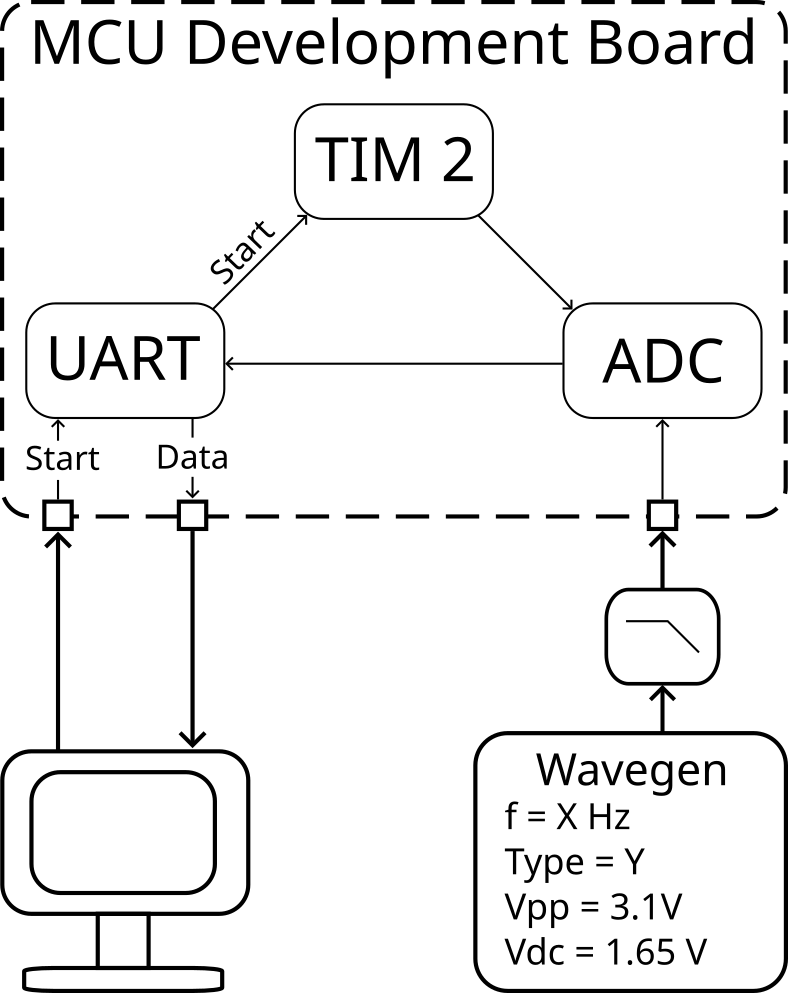
\includegraphics[width=0.9\linewidth]{figures/ADC_diagrama.png}
        \caption{\centering ADC}
    \end{subfigure}
    \begin{subfigure}{0.4\textwidth}
        \centering
        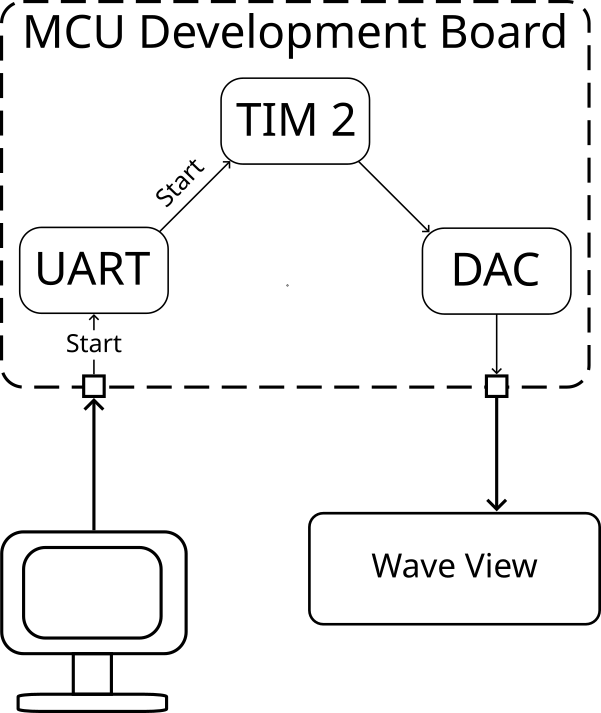
\includegraphics[width=0.9\linewidth]{figures/DAC_diagrama.png}
        \caption{\centering DAC}
    \end{subfigure}
    \caption{Entornos de trabajo utilizados para cada periférico}
    \label{fig:entorno}
\end{figure}
El firmware implementado para obtener las características del ADC y DAC mantiene una arquitectura de ejecución simple y directa, presentando leves diferencias operativas entre sí. En ambos casos, el proceso de medición se inicializa mediante el protocolo UART, enviando un dato de 8 bits de control (\texttt{0x01}) para dar inicio a la conversión. Posteriormente se activa el timer a utilizar (Timer 2 en el caso de la STM32). Transcurrido el tiempo de adquisición determinado por la cantidad de datos a medir, se detiene el timer y se da inicio al envío de datos mediante UART. Finalmente, esta información es procesada y 

 En ambos casos, el proceso se inicia de forma remota mediante el protocolo UART, enviando un dato de 8 bits de control (\texttt{0x01}) para dar inicio a la conversión. Posteriormente, se activan las interrupciones del Timer 2 para fijar una frecuencia de muestreo ( kHz para el ADC y 2Hz para el DAC). Transcurrido el tiempo de adquisición determinado (10 segundos para el ADC y cerca de 2.5 segundos para el DAC), las tramas de datos obtenidas se transmiten al computador mediante UART. Finalmente, esta información es procesada y tabulada a través de un \textit{script} de Python, encargado de extraer el comportamiento en corriente continua y calcular las métricas de error correspondientes frente al modelo ideal.
\\
Adicionalmente, se destaca que el firmware implementado para obtener las características de corriente alterna del ADC es el mismo para corriente continua.
%De manera similar, el firmware implementado para obtener las características de corriente alterna del ADC se mantiene idéntico, con la excepción de que se fija una frecuencia de muestreo de 100 kHz y ya no se utilizan interrupciones del Timer 2 para generar mediciones. Para lograr esto, se deshabilitan las interrupciones del Timer 2, se habilita el \textit{trigger} del ADC para que este opere mediante un evento por hardware del Timer 2 y, finalmente, se habilita la transferencia de datos continua por DMA.
\\
Finalmente, para poder medir la temperatura interna del microcontrolador, se hace uso del sensor de temperatura interno, el cual está conectado al ADC1 de la STM32, y de un secador de pelo que será utilizado para elevar la temperatura del microcontrolador al emanar calor directamente sobre el chip. Estas mediciones se realizan en un entorno de pruebas idéntico al de las mediciones de DC del ADC, esta vez utilizando el Timer 3 en lugar del Timer 2, y a una frecuencia de 2 Hz.
\section{Resultados}
Utilizando hasta 3 generadores de señales distintos para la obtención de métricas de corriente continua y 2 para corriente alterna, se obtuvieron las métricas de desempeño para los periféricos de señal mixta de la STM32 y ESP32. A continuación, se detallan los valores registrados para el convertidor análogo-digital (ADC) y el convertidor digital-análogo (DAC).
\subsection{Resultados del ADC (STM32)}
En la Tabla \ref{tab:Tabla STMADC DC} se presentan las métricas de corriente continua obtenidas para el ADC ante diversos generadores de señales. Dentro de las métricas de desempeño obtenidas, se destaca la métrica INL  y error de offset cuyos valores se desvían entre 5 a 10 veces de lo reportado en el datasheet para al menos dos generadores de señal
Destaca un error de offset de 25 LSB, valor que excede significativamente el rango de 2 a 4 LSB especificado en el \textit{datasheet} del fabricante. Por otro lado, el error de ganancia se registró en 1 LSB, situándose por debajo de los límites máximos esperados. En cuanto a las métricas de linealidad, el DNL se mantuvo cercano a la unidad (1.8 LSB máximo), mientras que el INL presentó una desviación de hasta 8 LSB.
\begin{table}[h]
    \centering
    \begin{tabular}{|l|c|c|c|c|}
        \hline
        \textbf{Métrica de desempeño} & \textbf{AD2} & \textbf{Tektronik CFG 280} &\textbf{Rigol DG1022} & \textbf{Datasheet} \\ \hline
        Error de Offset (LSB)  & 25         & 0.5   & 22.04 &[2 - 4]   \\ \hline
        Error de ganancia (LSB) & 1         & -1.18 & 1     &[4 - 4.5] \\ \hline
        INL (LSB)               & 4         & 21.74 & 14.56 &[2.5 - 3] \\ \hline
        DNL (LSB)               & 1.8       & 2.2   & 2.25  &[1 - 1.5] \\ \hline
    \end{tabular}
    \caption{Métricas de desempeño para el ADC del microcontrolador STM32L476RG.}
    \label{tab:Tabla STMADC DC}
\end{table}
Adicionalmente, en la tabla \ref{tab:Tabla STMADC AC} se presentan las métricas de desempeño de corriente continua obtenidas para el ADC ante dos generadores de señales distintos. Se destaca que todas las métricas obtenidas difieren considerablemente de lo reportado en el datasheet.
\begin{table}[h]
    \centering
    \begin{tabular}{|l|c|c|c|}
        \hline
        \textbf{Métrica de desempeño} & \textbf{AD2} & \textbf{Tektronik CFG 280} & \textbf{Datasheet} \\ \hline
        THD(db)     & -49.7      & -52.97 & -73   \\ \hline
        SINAD (db)  & 35.63      & 46.75  & 64.4 \\ \hline
        ENOB (bits) & 5.63       & 7.47   & 10.4 \\ \hline
    \end{tabular}
    \caption{Métricas de desempeño para el ADC del microcontrolador STM32L476RG.}
    \label{tab:Tabla STMADC AC}
\end{table}
\subsection{Resultados del DAC (STM32L476RG)}
Los resultados para el DAC, resumidos en la Tabla \ref{tab:Tabla STMDAC}, muestran una alta correlación con las especificaciones técnicas del componente. La ganancia obtenida fue de 0.479\%, muy cercana al 0.5\% nominal. Asimismo, los errores de offset medidos en los códigos \texttt{0x800} y \texttt{0x001} se mantuvieron en niveles mínimos (1 LSB y un rango de 1 a 2 LSB, respectivamente), ambos considerablemente menores a los valores máximos permitidos por el fabricante.
\begin{table}[h]
    \centering
    \begin{tabular}{|l|c|c|}
        \hline
        \textbf{Métrica de desempeño} & \textbf{Obtenida} & \textbf{Datasheet} \\ \hline
        Ganancia (\%)          & 0.479     & 0.5 \\ \hline
        Offset en 0x800 (LSB)  & 1         & 8   \\ \hline
        Offset en 0x001 (LSB)  & [1 - 2]   & 5   \\ \hline
    \end{tabular}
    \caption{Métricas de desempeño para el DAC de la STM32.}
    \label{tab:Tabla STMDAC}
\end{table}
\subsection{Mediciones a distintas temperaturas}
A estos resultados previos se suma la comparación de las métricas de corriente continua obtenidas con el Analog Discovery 2 a distintas temperaturas. En la tabla \ref{tab:dc adc temp}
\begin{table}[h]
    \centering
    \begin{tabular}{|l|c|c|}
        \hline
        \textbf{Métrica de desempeño} & \textbf{11°C} & \textbf{60°C} \\ \hline
        Error Ganancia (LSB)& 1         & 1.2 \\ \hline
        Error Offset (LSB)  & 17        & 39   \\ \hline
        INL (LSB)           & 8         & 25   \\ \hline
        DNL (LSB)           & 2         & 2.5 \\ \hline
    \end{tabular}
    \caption{Métricas DC de la STM32 ante 11°C y 60°C internos.}
    \label{tab:dc adc temp}
\end{table}
\subsection{Estado de la caracterización de la ESP32}
No se lograron consolidar mediciones para su inclusión en el presente informe de avance. Si bien, ya es posible generarlas y obtener métricas rudimentarias de su ADC, no se logró compatibilizar a tiempo esta tarjeta con el entorno de pruebas utilizado. Si bien se pudieron haber logrado obtener y reportar resultados de esta tarjeta de desarrollo a tiempo, se optó por no proceder por esa vía, pues se aspira a poder utilizar el mismo entorno de pruebas para ambas placas a modo de poder obtener una comparación en condiciones equivalentes.
\section{Discusión}
La caracterización realizada permite realizar un análisis crítico sobre el desempeño de los periféricos de señal mixta de la plataforma STM32 y la viabilidad del entorno de pruebas basado en el instrumental disponible.
\subsection{Análisis DC del ADC}
Una de las observaciones más significativas a realizar de este avance es la diferencia entre las métricas de desempeño obtenidas entre generadores de señales digitales y análogos, pues en los generadores digitales se nota una desviación significativa en el error de offset con respecto al datasheet, mientras que en los generadores análogos se observa un error de offset casi nulo, mientras que su error integral es el más alto entre los generadores observados, llegando a casi 7 veces el valor máximo especificado en el datasheet. Entre las causas posibles de esta diferencia existe el error de offset intrínseco del convertidor digital análogo del generador de señales digital, mientras que el generador de señales análogo, al ser un circuito no lineal en su rango máximo, se espera que no logre entregar una señal con un buen comportamiento esperado.
\subsection{Análisis AC del ADC}
Al evaluar el comportamiento dinámico del convertidor análogo-digital, expuesto en la Tabla 2, se observa una degradación severa en todas las métricas de corriente alterna en comparación a las especificaciones del fabricante. El Número Efectivo de Bits (ENOB) esperado según el \textit{datasheet} es de 10.4 bits; sin embargo, las mediciones arrojaron valores de apenas 5.63 bits utilizando el generador del Analog Discovery 2 y 7.47 bits empleando el Tektronik CFG 280. De manera correlacionada, la relación Señal a Ruido y Distorsión (SINAD) experimentó una caída drástica, registrando diferencias de entre 17 dB y 28 dB por debajo del valor ideal de 64.4 dB.
\\
Esta discrepancia sustancial no implica necesariamente un defecto o limitación en la arquitectura del microcontrolador, sino que evidencia una restricción fundamental en el banco de pruebas: la pureza espectral de los estímulos de entrada. Los generadores de señales utilizados poseen ruido de banda ancha y distorsión armónica intrínseca, defectos que el ADC de la STM32 está cuantificando de manera fidedigna. Es decir, el convertidor está caracterizando las limitaciones del instrumental más que sus propios límites.
\\
Adicionalmente, se debe considerar la respuesta en frecuencia del filtro antialiasing implementado. Si bien el filtro pasivo RC pasa-bajos establece una frecuencia de corte aproximada de 3.18 kHz, al ser de primer orden posee una pendiente de atenuación suave (20 dB/década). Al inyectar una señal fundamental en torno a los 1.2 kHz, el segundo armónico (2.4 kHz) pasa prácticamente sin atenuación hacia el microcontrolador, y el tercer armónico (3.6 kHz) es atenuado mínimamente. Esto justifica los deficientes niveles de THD obtenidos (-49.7 dB y -52.97 dB frente a los -73 dB especificados. Estos resultados demuestran la necesidad de contar con generadores de señal de baja distorsión o, en su defecto, implementar filtros activos de orden superior que logren atenuar los armónicos cercanos a la banda de paso antes del proceso de muestreo.
\subsection{Validación del DAC}
En contraste, el DAC del STM32 mostró una alta fidelidad frente a las especificaciones técnicas. Los resultados obtenidos para el error de ganancia (0.479\%) y los niveles de offset en diferentes códigos digitales se mantuvieron dentro de los márgenes de seguridad del fabricante[cite: 250, 253, 256]. Esto valida que la arquitectura R2R integrada es robusta y que el Analog Discovery 2 es un instrumento adecuado para la caracterización de este periférico en particular, dada su resolución superior de 14 bits[cite: 149, 197].
\subsection{Limitaciones y Trabajo Futuro}
Nuevamente, la principal limitación de este informe fue la falta de resultados para la tarjeta ESP32 S3 Mini. Esto atribuido a la necesidad de poder obtener métricas de desempeño bajo un entorno de pruebas unificado para la STM32 y ESP32.
\\
Como pasos a seguir para completar la investigación se propone:
\begin{itemize}
    \item Compatibilizar el firmware implementado en la tarjeta ESP32 S3 mini con el entorno de pruebas desarrollado para la tarjeta STM32 L475RG.
    \item Depurar exhaustivamente las métricas de desempeño de corriente alterna del ADC para corroborar que los datos obtenidos son representativos del sistema.
    \item Validar entorno de pruebas con 2 o más tarjetas STM32 L476RG con el propósito de depurar errores que el entorno de pruebas pueda tener y actualmente estén siendo ignoradas.
    \item Obtener todas las métricas planteadas para ambas tarjetas y a distintas temperaturas.
\end{itemize}
\printbibliography
\end{document}
